% Options for packages loaded elsewhere
\PassOptionsToPackage{unicode}{hyperref}
\PassOptionsToPackage{hyphens}{url}
%
\documentclass[
]{book}
\usepackage{lmodern}
\usepackage{amssymb,amsmath}
\usepackage{ifxetex,ifluatex}
\ifnum 0\ifxetex 1\fi\ifluatex 1\fi=0 % if pdftex
  \usepackage[T1]{fontenc}
  \usepackage[utf8]{inputenc}
  \usepackage{textcomp} % provide euro and other symbols
\else % if luatex or xetex
  \usepackage{unicode-math}
  \defaultfontfeatures{Scale=MatchLowercase}
  \defaultfontfeatures[\rmfamily]{Ligatures=TeX,Scale=1}
\fi
% Use upquote if available, for straight quotes in verbatim environments
\IfFileExists{upquote.sty}{\usepackage{upquote}}{}
\IfFileExists{microtype.sty}{% use microtype if available
  \usepackage[]{microtype}
  \UseMicrotypeSet[protrusion]{basicmath} % disable protrusion for tt fonts
}{}
\makeatletter
\@ifundefined{KOMAClassName}{% if non-KOMA class
  \IfFileExists{parskip.sty}{%
    \usepackage{parskip}
  }{% else
    \setlength{\parindent}{0pt}
    \setlength{\parskip}{6pt plus 2pt minus 1pt}}
}{% if KOMA class
  \KOMAoptions{parskip=half}}
\makeatother
\usepackage{xcolor}
\IfFileExists{xurl.sty}{\usepackage{xurl}}{} % add URL line breaks if available
\IfFileExists{bookmark.sty}{\usepackage{bookmark}}{\usepackage{hyperref}}
\hypersetup{
  pdftitle={Joe's R Guide},
  pdfauthor={Joe Mirza},
  hidelinks,
  pdfcreator={LaTeX via pandoc}}
\urlstyle{same} % disable monospaced font for URLs
\usepackage{color}
\usepackage{fancyvrb}
\newcommand{\VerbBar}{|}
\newcommand{\VERB}{\Verb[commandchars=\\\{\}]}
\DefineVerbatimEnvironment{Highlighting}{Verbatim}{commandchars=\\\{\}}
% Add ',fontsize=\small' for more characters per line
\usepackage{framed}
\definecolor{shadecolor}{RGB}{248,248,248}
\newenvironment{Shaded}{\begin{snugshade}}{\end{snugshade}}
\newcommand{\AlertTok}[1]{\textcolor[rgb]{0.94,0.16,0.16}{#1}}
\newcommand{\AnnotationTok}[1]{\textcolor[rgb]{0.56,0.35,0.01}{\textbf{\textit{#1}}}}
\newcommand{\AttributeTok}[1]{\textcolor[rgb]{0.77,0.63,0.00}{#1}}
\newcommand{\BaseNTok}[1]{\textcolor[rgb]{0.00,0.00,0.81}{#1}}
\newcommand{\BuiltInTok}[1]{#1}
\newcommand{\CharTok}[1]{\textcolor[rgb]{0.31,0.60,0.02}{#1}}
\newcommand{\CommentTok}[1]{\textcolor[rgb]{0.56,0.35,0.01}{\textit{#1}}}
\newcommand{\CommentVarTok}[1]{\textcolor[rgb]{0.56,0.35,0.01}{\textbf{\textit{#1}}}}
\newcommand{\ConstantTok}[1]{\textcolor[rgb]{0.00,0.00,0.00}{#1}}
\newcommand{\ControlFlowTok}[1]{\textcolor[rgb]{0.13,0.29,0.53}{\textbf{#1}}}
\newcommand{\DataTypeTok}[1]{\textcolor[rgb]{0.13,0.29,0.53}{#1}}
\newcommand{\DecValTok}[1]{\textcolor[rgb]{0.00,0.00,0.81}{#1}}
\newcommand{\DocumentationTok}[1]{\textcolor[rgb]{0.56,0.35,0.01}{\textbf{\textit{#1}}}}
\newcommand{\ErrorTok}[1]{\textcolor[rgb]{0.64,0.00,0.00}{\textbf{#1}}}
\newcommand{\ExtensionTok}[1]{#1}
\newcommand{\FloatTok}[1]{\textcolor[rgb]{0.00,0.00,0.81}{#1}}
\newcommand{\FunctionTok}[1]{\textcolor[rgb]{0.00,0.00,0.00}{#1}}
\newcommand{\ImportTok}[1]{#1}
\newcommand{\InformationTok}[1]{\textcolor[rgb]{0.56,0.35,0.01}{\textbf{\textit{#1}}}}
\newcommand{\KeywordTok}[1]{\textcolor[rgb]{0.13,0.29,0.53}{\textbf{#1}}}
\newcommand{\NormalTok}[1]{#1}
\newcommand{\OperatorTok}[1]{\textcolor[rgb]{0.81,0.36,0.00}{\textbf{#1}}}
\newcommand{\OtherTok}[1]{\textcolor[rgb]{0.56,0.35,0.01}{#1}}
\newcommand{\PreprocessorTok}[1]{\textcolor[rgb]{0.56,0.35,0.01}{\textit{#1}}}
\newcommand{\RegionMarkerTok}[1]{#1}
\newcommand{\SpecialCharTok}[1]{\textcolor[rgb]{0.00,0.00,0.00}{#1}}
\newcommand{\SpecialStringTok}[1]{\textcolor[rgb]{0.31,0.60,0.02}{#1}}
\newcommand{\StringTok}[1]{\textcolor[rgb]{0.31,0.60,0.02}{#1}}
\newcommand{\VariableTok}[1]{\textcolor[rgb]{0.00,0.00,0.00}{#1}}
\newcommand{\VerbatimStringTok}[1]{\textcolor[rgb]{0.31,0.60,0.02}{#1}}
\newcommand{\WarningTok}[1]{\textcolor[rgb]{0.56,0.35,0.01}{\textbf{\textit{#1}}}}
\usepackage{longtable,booktabs}
% Correct order of tables after \paragraph or \subparagraph
\usepackage{etoolbox}
\makeatletter
\patchcmd\longtable{\par}{\if@noskipsec\mbox{}\fi\par}{}{}
\makeatother
% Allow footnotes in longtable head/foot
\IfFileExists{footnotehyper.sty}{\usepackage{footnotehyper}}{\usepackage{footnote}}
\makesavenoteenv{longtable}
\usepackage{graphicx,grffile}
\makeatletter
\def\maxwidth{\ifdim\Gin@nat@width>\linewidth\linewidth\else\Gin@nat@width\fi}
\def\maxheight{\ifdim\Gin@nat@height>\textheight\textheight\else\Gin@nat@height\fi}
\makeatother
% Scale images if necessary, so that they will not overflow the page
% margins by default, and it is still possible to overwrite the defaults
% using explicit options in \includegraphics[width, height, ...]{}
\setkeys{Gin}{width=\maxwidth,height=\maxheight,keepaspectratio}
% Set default figure placement to htbp
\makeatletter
\def\fps@figure{htbp}
\makeatother
\setlength{\emergencystretch}{3em} % prevent overfull lines
\providecommand{\tightlist}{%
  \setlength{\itemsep}{0pt}\setlength{\parskip}{0pt}}
\setcounter{secnumdepth}{5}
\usepackage{booktabs}
\usepackage[]{natbib}
\bibliographystyle{apalike}

\title{Joe's R Guide}
\author{Joe Mirza}
\date{2021-06-04}

\begin{document}
\maketitle

{
\setcounter{tocdepth}{1}
\tableofcontents
}
\hypertarget{r-studio-environment}{%
\chapter{R Studio Environment}\label{r-studio-environment}}

Understanding the R Studio environment.

This is a \emph{sample} book written in \textbf{Markdown}. You can use anything that Pandoc's Markdown supports, e.g., a math equation \(a^2 + b^2 = c^2\).

The \textbf{bookdown} package can be installed from CRAN or Github:

\begin{Shaded}
\begin{Highlighting}[]
\KeywordTok{install.packages}\NormalTok{(}\StringTok{"bookdown"}\NormalTok{)}
\KeywordTok{library}\NormalTok{(tinytex)}
\KeywordTok{library}\NormalTok{(tidyverse)}
\CommentTok{# or the development version}
\CommentTok{# devtools::install_github("rstudio/bookdown")}
\end{Highlighting}
\end{Shaded}

Remember each Rmd file contains one and only one chapter, and a chapter is defined by the first-level heading \texttt{\#}.

To compile this example to PDF, you need XeLaTeX. You are recommended to install TinyTeX (which includes XeLaTeX): \url{https://yihui.org/tinytex/}.

\hypertarget{r-studio-vs.-r-and-r-markdown}{%
\section{R Studio vs.~R and R Markdown}\label{r-studio-vs.-r-and-r-markdown}}

The file type this is being written in is called R Markdown. It's a Markdown file that\\
lets you insert and run R code in two types of places that are\ldots not Markdown.

The first type is a code chunk. It looks like this:

\begin{verbatim}
```{r}

```
\end{verbatim}

This is the most minimal sort of chunk. Three backticks, followed by r in brackets,
ending in three backticks. Other instructions can follow the \texttt{r}. The most commonly used ones are:

\begin{enumerate}
\def\labelenumi{\arabic{enumi}.}
\item
  Instructions that suppress certain types of content from being displayed
  (e.g.~\texttt{echo\ =\ FALSE} means prevents code, but not the results from appearing in the finished file.)
\item
  Captions for graphical results using \texttt{fig.cap\ =\ "..."}.
\item
  The ability to set the size and layout of the images. Much more about this in
  plotting.
\end{enumerate}

Link to specifics here: \href{https://rmarkdown.rstudio.com/lesson-3.html}{Code Chunks}

The other way you can insert R code into your markdown is `inline'. Say you had a numeric variable you'd calculated above called \texttt{varname} and wanted to use the value inline. You'd do that like so:

\begin{verbatim}
`r varname`
\end{verbatim}

Where the numeric value of \texttt{varname} would be inserted in that location.

\hypertarget{rstudio-and-the-file-system}{%
\section{RStudio and the File System}\label{rstudio-and-the-file-system}}

\begin{itemize}
\item
  Get the working directory: \texttt{getwd()}
\item
  Set the working directory: \texttt{setwd("/home/jovyan/RBridge/")}
\item
  Note that by hitting backslash in rstudio, it will provide you options for the
  next directory in the file hierarchy
\item
  List of files in current working directory: \texttt{list.files()}
\end{itemize}

\hypertarget{ls-vs.-list.files}{%
\section{\texorpdfstring{\texttt{ls()} vs.~\texttt{list.files()}}{ls() vs.~list.files()}}\label{ls-vs.-list.files}}

\begin{itemize}
\item
  \texttt{ls()} gives you the list of variables in the global environment.
\item
  If you want to clear the local environmental variables, you would type \texttt{rm(list\ =\ ls())}. You probably could be forgiven for thinking it would've been \texttt{rm(ls())}, but no dice!
\item
  Note that \texttt{ls()} is different from \texttt{list.files()}. \texttt{list.files()} lists the files in the \emph{working directory}. \texttt{ls()} provides the variables in \emph{working memory}.
\end{itemize}

\hypertarget{handy-shortcuts}{%
\section{Handy Shortcuts}\label{handy-shortcuts}}

\textbf{Changing Focus between Source and Console Panels}

\begin{itemize}
\item
  To change focus to the source (where you write the code as full-fledged scripts): \texttt{ctrl-1}
\item
  To change focus to the console (where you see the output or write one-off commands): \texttt{ctrl-2}
\end{itemize}

\textbf{What kind of object is this? (e.g.~data.frame, data.table, vector?)}

\begin{Shaded}
\begin{Highlighting}[]
  \KeywordTok{typeof}\NormalTok{(squirrel_subset)}
\end{Highlighting}
\end{Shaded}

\begin{verbatim}
## [1] "list"
\end{verbatim}

\begin{Shaded}
\begin{Highlighting}[]
  \KeywordTok{class}\NormalTok{(squirrel_subset)}
\end{Highlighting}
\end{Shaded}

\begin{verbatim}
## [1] "data.frame"
\end{verbatim}

\textbf{Comment/Uncomment Code:}

\begin{verbatim}
`shift + command + C`
\end{verbatim}

\textbf{Keyboard shortcut to insert a code chunk:}

\begin{verbatim}
`Cmd + Option + I`

Gives you an empty code chunk:

```{r}

```
\end{verbatim}

Also note how one can display the code for a code chunk and not the result.(Look in the source code to see how.)

\textbf{Getting Help}

\begin{itemize}
\item
  You can use \texttt{?} before a command to get help on a topic. For example:
  \texttt{?geom\_point} returns a help page for that topic.
\item
  You can also type \texttt{help(geom\_point)} to achieve the same effect.
\end{itemize}

\textbf{Installing and Loading Packages}

\begin{itemize}
\item
  To install a package (note the quotes around \texttt{zoo}): \texttt{install.packages(\textquotesingle{}zoo\textquotesingle{})}
\item
  To load that package and make it available (no quotes): \texttt{library(zoo)}
\item
  The \texttt{::} specifies the package an object comes from, for example: \texttt{dplyr::mutate()}
\end{itemize}

\textbf{Clearing the console:} \texttt{Ctrl-L}.

\hypertarget{intro}{%
\chapter{Summary \& Overview Functions}\label{intro}}

Basic dataframe for some of the examples below.

\begin{Shaded}
\begin{Highlighting}[]
\NormalTok{d <-}\StringTok{ }\KeywordTok{data.frame}\NormalTok{(     }
  \DataTypeTok{id =} \DecValTok{1}\OperatorTok{:}\DecValTok{1000}\NormalTok{,     }
  \DataTypeTok{x =} \KeywordTok{rnorm}\NormalTok{(}\DecValTok{1000}\NormalTok{, }\DataTypeTok{mean =} \DecValTok{0}\NormalTok{, }\DataTypeTok{sd =} \DecValTok{1}\NormalTok{),    }
  \DataTypeTok{y =} \KeywordTok{rnorm}\NormalTok{(}\DecValTok{1000}\NormalTok{, }\DataTypeTok{mean =} \DecValTok{10}\NormalTok{, }\DataTypeTok{sd =} \DecValTok{2}\NormalTok{),     }
  \DataTypeTok{color =} \KeywordTok{sample}\NormalTok{(}\KeywordTok{c}\NormalTok{(}\StringTok{'red'}\NormalTok{, }\StringTok{'blue'}\NormalTok{), }\DataTypeTok{size =} \DecValTok{1000}\NormalTok{, }\DataTypeTok{replace =} \OtherTok{TRUE}\NormalTok{)    }
\NormalTok{) }
\end{Highlighting}
\end{Shaded}

You can label chapter and section titles using \texttt{\{\#label\}} after them, e.g., we can reference Chapter \ref{intro}. If you do not manually label them, there will be automatic labels anyway, e.g., Chapter \ref{methods}.

Figures and tables with captions will be placed in \texttt{figure} and \texttt{table} environments, respectively.

\begin{Shaded}
\begin{Highlighting}[]
\KeywordTok{par}\NormalTok{(}\DataTypeTok{mar =} \KeywordTok{c}\NormalTok{(}\DecValTok{4}\NormalTok{, }\DecValTok{4}\NormalTok{, }\FloatTok{.1}\NormalTok{, }\FloatTok{.1}\NormalTok{))}
\KeywordTok{plot}\NormalTok{(pressure, }\DataTypeTok{type =} \StringTok{'b'}\NormalTok{, }\DataTypeTok{pch =} \DecValTok{19}\NormalTok{)}
\end{Highlighting}
\end{Shaded}

\begin{figure}

{\centering 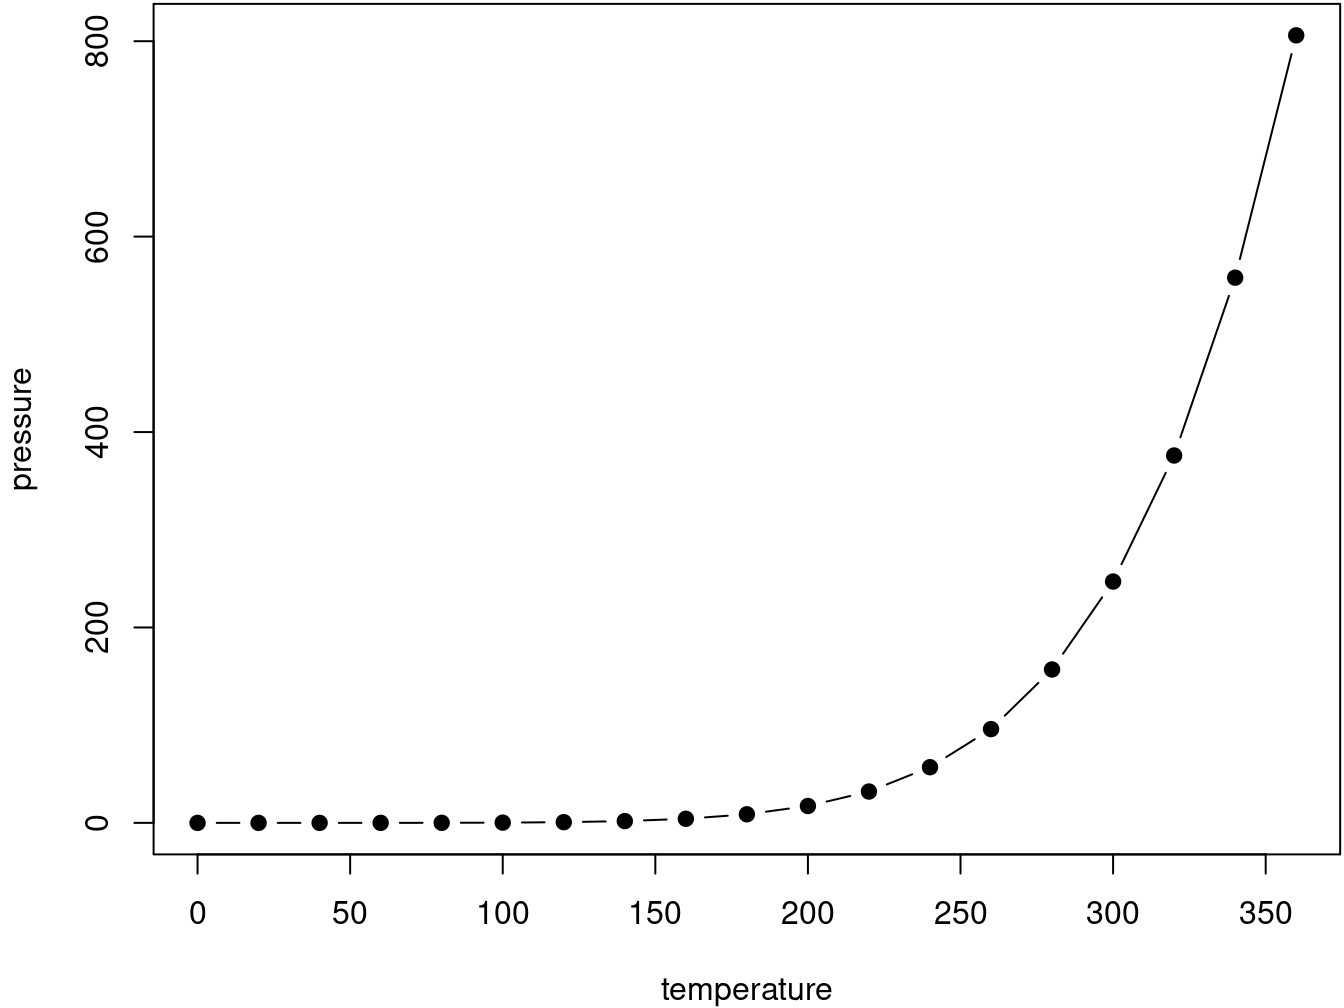
\includegraphics[width=0.8\linewidth]{Joes_R_Guide_files/figure-latex/nice-fig-1} 

}

\caption{Here is a nice figure!}\label{fig:nice-fig}
\end{figure}

Reference a figure by its code chunk label with the \texttt{fig:} prefix, e.g., see Figure \ref{fig:nice-fig}. Similarly, you can reference tables generated from \texttt{knitr::kable()}, e.g., see Table \ref{tab:nice-tab}.

\begin{Shaded}
\begin{Highlighting}[]
\NormalTok{knitr}\OperatorTok{::}\KeywordTok{kable}\NormalTok{(}
  \KeywordTok{head}\NormalTok{(iris, }\DecValTok{20}\NormalTok{), }\DataTypeTok{caption =} \StringTok{'Here is a nice table!'}\NormalTok{,}
  \DataTypeTok{booktabs =} \OtherTok{TRUE}
\NormalTok{)}
\end{Highlighting}
\end{Shaded}

\begin{table}

\caption{\label{tab:nice-tab}Here is a nice table!}
\centering
\begin{tabular}[t]{rrrrl}
\toprule
Sepal.Length & Sepal.Width & Petal.Length & Petal.Width & Species\\
\midrule
5.1 & 3.5 & 1.4 & 0.2 & setosa\\
4.9 & 3.0 & 1.4 & 0.2 & setosa\\
4.7 & 3.2 & 1.3 & 0.2 & setosa\\
4.6 & 3.1 & 1.5 & 0.2 & setosa\\
5.0 & 3.6 & 1.4 & 0.2 & setosa\\
\addlinespace
5.4 & 3.9 & 1.7 & 0.4 & setosa\\
4.6 & 3.4 & 1.4 & 0.3 & setosa\\
5.0 & 3.4 & 1.5 & 0.2 & setosa\\
4.4 & 2.9 & 1.4 & 0.2 & setosa\\
4.9 & 3.1 & 1.5 & 0.1 & setosa\\
\addlinespace
5.4 & 3.7 & 1.5 & 0.2 & setosa\\
4.8 & 3.4 & 1.6 & 0.2 & setosa\\
4.8 & 3.0 & 1.4 & 0.1 & setosa\\
4.3 & 3.0 & 1.1 & 0.1 & setosa\\
5.8 & 4.0 & 1.2 & 0.2 & setosa\\
\addlinespace
5.7 & 4.4 & 1.5 & 0.4 & setosa\\
5.4 & 3.9 & 1.3 & 0.4 & setosa\\
5.1 & 3.5 & 1.4 & 0.3 & setosa\\
5.7 & 3.8 & 1.7 & 0.3 & setosa\\
5.1 & 3.8 & 1.5 & 0.3 & setosa\\
\bottomrule
\end{tabular}
\end{table}

You can write citations, too. For example, we are using the \textbf{bookdown} package \citep{R-bookdown} in this sample book, which was built on top of R Markdown and \textbf{knitr} \citep{xie2015}.

\hypertarget{rstudio-cheatsheets-master-list}{%
\section{\texorpdfstring{\href{https://www.rstudio.com/resources/cheatsheets/}{RStudio Cheatsheets (master list)}}{RStudio Cheatsheets (master list)}}\label{rstudio-cheatsheets-master-list}}

These seem handy.

Some functions that can give you a sense of the data you're working with.

List of these functions:\\
- \texttt{summary}
- \texttt{glimpse}

\begin{itemize}
\tightlist
\item
  \texttt{table}
\item
  \texttt{dim}~\\
\item
  \texttt{nrow}~\\
\item
  \texttt{ncol}~\\
\item
  \texttt{count}~\\
\item
  \texttt{names}
\end{itemize}

\hypertarget{summary}{%
\section{\texorpdfstring{\texttt{summary}}{summary}}\label{summary}}

Provides a summary of each data series in a dataframe. Good for getting a sense of the range of the
data as well as outliers and missing values.

\begin{Shaded}
\begin{Highlighting}[]
\KeywordTok{summary}\NormalTok{(nyc_license)}
\end{Highlighting}
\end{Shaded}

\begin{verbatim}
##  animal_name        animal_gender      animal_birth_month     breed_rc        
##  Length:122203      Length:122203      Min.   :1999-01-01   Length:122203     
##  Class :character   Class :character   1st Qu.:2007-10-01   Class :character  
##  Mode  :character   Mode  :character   Median :2011-05-01   Mode  :character  
##                                        Mean   :2010-09-05                     
##                                        3rd Qu.:2014-05-01                     
##                                        Max.   :2017-03-01                     
##                                                                               
##    borough             zip_code     community_district census_tract2010
##  Length:122203      Min.   :  121   Min.   :101.0      Min.   :     1  
##  Class :character   1st Qu.:10029   1st Qu.:108.0      1st Qu.:   126  
##  Mode  :character   Median :10465   Median :302.0      Median :   251  
##                     Mean   :10678   Mean   :265.2      Mean   :  7339  
##                     3rd Qu.:11228   3rd Qu.:403.0      3rd Qu.:   912  
##                     Max.   :94608   Max.   :595.0      Max.   :157903  
##                                     NA's   :3341       NA's   :3341    
##      nta            city_council_district congressional_district
##  Length:122203      Min.   : 1.00         Min.   : 3.00         
##  Class :character   1st Qu.: 6.00         1st Qu.: 8.00         
##  Mode  :character   Median :22.00         Median :11.00         
##                     Mean   :22.83         Mean   :10.27         
##                     3rd Qu.:37.00         3rd Qu.:12.00         
##                     Max.   :51.00         Max.   :16.00         
##                     NA's   :3341          NA's   :3341          
##  state_senatorial_district license_issued_date  license_expired_date
##  Min.   :10.00             Min.   :2014-09-12   Min.   :2016-01-01  
##  1st Qu.:18.00             1st Qu.:2015-08-24   1st Qu.:2016-10-13  
##  Median :25.00             Median :2016-03-25   Median :2017-05-07  
##  Mean   :23.54             Mean   :2016-02-13   Mean   :2017-05-24  
##  3rd Qu.:28.00             3rd Qu.:2016-07-30   3rd Qu.:2017-09-27  
##  Max.   :36.00             Max.   :2016-12-31   Max.   :2022-11-20  
##  NA's   :3341              NA's   :1
\end{verbatim}

\texttt{summary} behaves differently depending on the objects it's applied to:

Above we ran summary on the dataframe \texttt{nyc\_license}. Here we can create a model \texttt{mod}.
We can run the \texttt{summary} function on each and get very different results.

\begin{Shaded}
\begin{Highlighting}[]
\NormalTok{mod <-}\StringTok{ }\KeywordTok{lm}\NormalTok{(y }\OperatorTok{~}\StringTok{ }\NormalTok{x, }\DataTypeTok{data =}\NormalTok{ d)}

\KeywordTok{summary}\NormalTok{(d)}
\end{Highlighting}
\end{Shaded}

\begin{verbatim}
##        id               x                  y             color          
##  Min.   :   1.0   Min.   :-2.75003   Min.   : 4.356   Length:1000       
##  1st Qu.: 250.8   1st Qu.:-0.60807   1st Qu.: 8.563   Class :character  
##  Median : 500.5   Median : 0.02130   Median : 9.988   Mode  :character  
##  Mean   : 500.5   Mean   : 0.05543   Mean   : 9.997                     
##  3rd Qu.: 750.2   3rd Qu.: 0.70286   3rd Qu.:11.375                     
##  Max.   :1000.0   Max.   : 4.00969   Max.   :16.240
\end{verbatim}

\begin{Shaded}
\begin{Highlighting}[]
\KeywordTok{summary}\NormalTok{(mod)}
\end{Highlighting}
\end{Shaded}

\begin{verbatim}
## 
## Call:
## lm(formula = y ~ x, data = d)
## 
## Residuals:
##     Min      1Q  Median      3Q     Max 
## -5.6339 -1.4383 -0.0123  1.3899  6.2329 
## 
## Coefficients:
##             Estimate Std. Error t value Pr(>|t|)    
## (Intercept)  9.99781    0.06441 155.216   <2e-16 ***
## x           -0.01059    0.06491  -0.163     0.87    
## ---
## Signif. codes:  0 '***' 0.001 '**' 0.01 '*' 0.05 '.' 0.1 ' ' 1
## 
## Residual standard error: 2.034 on 998 degrees of freedom
## Multiple R-squared:  2.667e-05,  Adjusted R-squared:  -0.0009753 
## F-statistic: 0.02662 on 1 and 998 DF,  p-value: 0.8704
\end{verbatim}

\hypertarget{print-glimpse-str}{%
\section{\texorpdfstring{\texttt{print}, \texttt{glimpse} \& \texttt{str}}{print, glimpse \& str}}\label{print-glimpse-str}}

Alternative ways to see the contents of the data in more detail than \texttt{summary()} provides.

\begin{Shaded}
\begin{Highlighting}[]
\KeywordTok{print}\NormalTok{(mpg)}
\end{Highlighting}
\end{Shaded}

\begin{verbatim}
## # A tibble: 234 x 11
##    manufacturer model    displ  year   cyl trans   drv     cty   hwy fl    class
##    <chr>        <chr>    <dbl> <int> <int> <chr>   <chr> <int> <int> <chr> <chr>
##  1 audi         a4         1.8  1999     4 auto(l~ f        18    29 p     comp~
##  2 audi         a4         1.8  1999     4 manual~ f        21    29 p     comp~
##  3 audi         a4         2    2008     4 manual~ f        20    31 p     comp~
##  4 audi         a4         2    2008     4 auto(a~ f        21    30 p     comp~
##  5 audi         a4         2.8  1999     6 auto(l~ f        16    26 p     comp~
##  6 audi         a4         2.8  1999     6 manual~ f        18    26 p     comp~
##  7 audi         a4         3.1  2008     6 auto(a~ f        18    27 p     comp~
##  8 audi         a4 quat~   1.8  1999     4 manual~ 4        18    26 p     comp~
##  9 audi         a4 quat~   1.8  1999     4 auto(l~ 4        16    25 p     comp~
## 10 audi         a4 quat~   2    2008     4 manual~ 4        20    28 p     comp~
## # ... with 224 more rows
\end{verbatim}

Note that the data type is also included.

\begin{Shaded}
\begin{Highlighting}[]
\KeywordTok{glimpse}\NormalTok{(mpg)}
\end{Highlighting}
\end{Shaded}

\begin{verbatim}
## Rows: 234
## Columns: 11
## $ manufacturer <chr> "audi", "audi", "audi", "audi", "audi", "audi", "audi", "~
## $ model        <chr> "a4", "a4", "a4", "a4", "a4", "a4", "a4", "a4 quattro", "~
## $ displ        <dbl> 1.8, 1.8, 2.0, 2.0, 2.8, 2.8, 3.1, 1.8, 1.8, 2.0, 2.0, 2.~
## $ year         <int> 1999, 1999, 2008, 2008, 1999, 1999, 2008, 1999, 1999, 200~
## $ cyl          <int> 4, 4, 4, 4, 6, 6, 6, 4, 4, 4, 4, 6, 6, 6, 6, 6, 6, 8, 8, ~
## $ trans        <chr> "auto(l5)", "manual(m5)", "manual(m6)", "auto(av)", "auto~
## $ drv          <chr> "f", "f", "f", "f", "f", "f", "f", "4", "4", "4", "4", "4~
## $ cty          <int> 18, 21, 20, 21, 16, 18, 18, 18, 16, 20, 19, 15, 17, 17, 1~
## $ hwy          <int> 29, 29, 31, 30, 26, 26, 27, 26, 25, 28, 27, 25, 25, 25, 2~
## $ fl           <chr> "p", "p", "p", "p", "p", "p", "p", "p", "p", "p", "p", "p~
## $ class        <chr> "compact", "compact", "compact", "compact", "compact", "c~
\end{verbatim}

\begin{Shaded}
\begin{Highlighting}[]
\KeywordTok{str}\NormalTok{(mpg)}
\end{Highlighting}
\end{Shaded}

\begin{verbatim}
## tibble[,11] [234 x 11] (S3: tbl_df/tbl/data.frame)
##  $ manufacturer: chr [1:234] "audi" "audi" "audi" "audi" ...
##  $ model       : chr [1:234] "a4" "a4" "a4" "a4" ...
##  $ displ       : num [1:234] 1.8 1.8 2 2 2.8 2.8 3.1 1.8 1.8 2 ...
##  $ year        : int [1:234] 1999 1999 2008 2008 1999 1999 2008 1999 1999 2008 ...
##  $ cyl         : int [1:234] 4 4 4 4 6 6 6 4 4 4 ...
##  $ trans       : chr [1:234] "auto(l5)" "manual(m5)" "manual(m6)" "auto(av)" ...
##  $ drv         : chr [1:234] "f" "f" "f" "f" ...
##  $ cty         : int [1:234] 18 21 20 21 16 18 18 18 16 20 ...
##  $ hwy         : int [1:234] 29 29 31 30 26 26 27 26 25 28 ...
##  $ fl          : chr [1:234] "p" "p" "p" "p" ...
##  $ class       : chr [1:234] "compact" "compact" "compact" "compact" ...
\end{verbatim}

(I think \texttt{str()} might have some powers beyond the above to unpack R objects.)

\hypertarget{dim-row-and-col}{%
\section{\texorpdfstring{\texttt{dim}, \texttt{row} and \texttt{col}}{dim, row and col}}\label{dim-row-and-col}}

Shape, rows and columns of dataframe:

\begin{Shaded}
\begin{Highlighting}[]
\KeywordTok{dim}\NormalTok{(nyc_license)}
\end{Highlighting}
\end{Shaded}

\begin{verbatim}
## [1] 122203     14
\end{verbatim}

\begin{Shaded}
\begin{Highlighting}[]
\KeywordTok{nrow}\NormalTok{(nyc_license)}
\end{Highlighting}
\end{Shaded}

\begin{verbatim}
## [1] 122203
\end{verbatim}

\begin{Shaded}
\begin{Highlighting}[]
\KeywordTok{ncol}\NormalTok{(nyc_license)}
\end{Highlighting}
\end{Shaded}

\begin{verbatim}
## [1] 14
\end{verbatim}

\hypertarget{count}{%
\section{\texorpdfstring{\texttt{count()}}{count()}}\label{count}}

Useful count of unique combinations.
Easiest to understand with an example:

\begin{Shaded}
\begin{Highlighting}[]
\KeywordTok{count}\NormalTok{(mpg,manufacturer, class)}
\end{Highlighting}
\end{Shaded}

\begin{verbatim}
## # A tibble: 32 x 3
##    manufacturer class          n
##    <chr>        <chr>      <int>
##  1 audi         compact       15
##  2 audi         midsize        3
##  3 chevrolet    2seater        5
##  4 chevrolet    midsize        5
##  5 chevrolet    suv            9
##  6 dodge        minivan       11
##  7 dodge        pickup        19
##  8 dodge        suv            7
##  9 ford         pickup         7
## 10 ford         subcompact     9
## # ... with 22 more rows
\end{verbatim}

chevrolet has 5 different 2 seaters across the dataset. Using \texttt{filter}, you can
see these are 5 different corvettes:

\begin{Shaded}
\begin{Highlighting}[]
\KeywordTok{filter}\NormalTok{(mpg,manufacturer}\OperatorTok{==}\StringTok{"chevrolet"}\NormalTok{, class}\OperatorTok{==}\StringTok{"2seater"}\NormalTok{ )}
\end{Highlighting}
\end{Shaded}

\begin{verbatim}
## # A tibble: 5 x 11
##   manufacturer model   displ  year   cyl trans    drv     cty   hwy fl    class 
##   <chr>        <chr>   <dbl> <int> <int> <chr>    <chr> <int> <int> <chr> <chr> 
## 1 chevrolet    corvet~   5.7  1999     8 manual(~ r        16    26 p     2seat~
## 2 chevrolet    corvet~   5.7  1999     8 auto(l4) r        15    23 p     2seat~
## 3 chevrolet    corvet~   6.2  2008     8 manual(~ r        16    26 p     2seat~
## 4 chevrolet    corvet~   6.2  2008     8 auto(s6) r        15    25 p     2seat~
## 5 chevrolet    corvet~   7    2008     8 manual(~ r        15    24 p     2seat~
\end{verbatim}

\hypertarget{table}{%
\section{\texorpdfstring{\texttt{table()}}{table()}}\label{table}}

\texttt{table()} is similar to \texttt{count()}, but provides you with the counts for all possible
combinations, even if the value is 0.

\begin{Shaded}
\begin{Highlighting}[]
\KeywordTok{table}\NormalTok{(mpg}\OperatorTok{$}\NormalTok{manufacturer, mpg}\OperatorTok{$}\NormalTok{class)}
\end{Highlighting}
\end{Shaded}

\begin{verbatim}
##             
##              2seater compact midsize minivan pickup subcompact suv
##   audi             0      15       3       0      0          0   0
##   chevrolet        5       0       5       0      0          0   9
##   dodge            0       0       0      11     19          0   7
##   ford             0       0       0       0      7          9   9
##   honda            0       0       0       0      0          9   0
##   hyundai          0       0       7       0      0          7   0
##   jeep             0       0       0       0      0          0   8
##   land rover       0       0       0       0      0          0   4
##   lincoln          0       0       0       0      0          0   3
##   mercury          0       0       0       0      0          0   4
##   nissan           0       2       7       0      0          0   4
##   pontiac          0       0       5       0      0          0   0
##   subaru           0       4       0       0      0          4   6
##   toyota           0      12       7       0      7          0   8
##   volkswagen       0      14       7       0      0          6   0
\end{verbatim}

\hypertarget{head-and-tail-functions-in-r}{%
\section{\texorpdfstring{\texttt{head()} and \texttt{tail()} Functions in R}{head() and tail() Functions in R}}\label{head-and-tail-functions-in-r}}

\begin{Shaded}
\begin{Highlighting}[]
\KeywordTok{head}\NormalTok{(d, }\DecValTok{5}\NormalTok{) }\CommentTok{# where d is dataframe}
\end{Highlighting}
\end{Shaded}

\begin{verbatim}
##   id          x         y color
## 1  1 -0.3644521 11.018493   red
## 2  2  1.5566929 11.939726   red
## 3  3 -0.1567763  9.658720  blue
## 4  4 -0.5055430  7.377748  blue
## 5  5  2.8971199  7.573144   red
\end{verbatim}

\begin{Shaded}
\begin{Highlighting}[]
\KeywordTok{tail}\NormalTok{(d, }\DecValTok{5}\NormalTok{)}
\end{Highlighting}
\end{Shaded}

Not that by including 'results=``hide'' in the code chunk, the code is displayed but the results are not.

\hypertarget{names}{%
\section{\texorpdfstring{\texttt{names()}}{names()}}\label{names}}

\texttt{names} isn't a particularly useful overview function, but it can be useful to
pull column headings in a vector, which can then be referenced like any other vector.

\begin{Shaded}
\begin{Highlighting}[]
\KeywordTok{names}\NormalTok{(nyc_license)}
\end{Highlighting}
\end{Shaded}

\begin{verbatim}
##  [1] "animal_name"               "animal_gender"            
##  [3] "animal_birth_month"        "breed_rc"                 
##  [5] "borough"                   "zip_code"                 
##  [7] "community_district"        "census_tract2010"         
##  [9] "nta"                       "city_council_district"    
## [11] "congressional_district"    "state_senatorial_district"
## [13] "license_issued_date"       "license_expired_date"
\end{verbatim}

\begin{Shaded}
\begin{Highlighting}[]
\KeywordTok{names}\NormalTok{(nyc_license)[}\DecValTok{3}\NormalTok{]}
\end{Highlighting}
\end{Shaded}

\begin{verbatim}
## [1] "animal_birth_month"
\end{verbatim}

\hypertarget{vectors}{%
\chapter{Vectors}\label{vectors}}

Primary Source:

\href{https://r4ds.had.co.nz/vectors.html}{R for Data Science: Vectors}

\hypertarget{vector-basics}{%
\section{Vector basics}\label{vector-basics}}

In some ways, working with vectors is harder than working with dataframes and data tables.
That's slightly counterintuitive, as they're the most atomic unit one works with in R. In Manning's
*Practical Data Science with R` they state:

\begin{quote}
\emph{"R's most basic data type is the vector, or array\ldots.R is fairly unique in having no scalar types. A single number such as the number 5 is represented in R as a vector with exactly one entry (5).}
\end{quote}

There are two types of vectors:

\begin{enumerate}
\def\labelenumi{\arabic{enumi}.}
\item
  \textbf{Atomic} vectors, of which there are six types: \textbf{logical}, \textbf{integer}, \textbf{double}, \textbf{character}, \textbf{complex}, and \textbf{raw}.
  Integer and double vectors are collectively known as \textbf{numeric} vectors.
\item
  \textbf{Lists}, which are sometimes called recursive vectors because lists can contain other lists.
\end{enumerate}

The chief difference between atomic vectors and lists is that atomic vectors are homogeneous, while lists can be heterogeneous. There's one other related object: NULL. NULL is often used to represent the absence of a vector (as opposed to NA which is used to represent the absence of a value in a vector). NULL typically behaves like a vector of length 0. Figure 20.1 summarises the interrelationships.

\begin{figure}
\centering
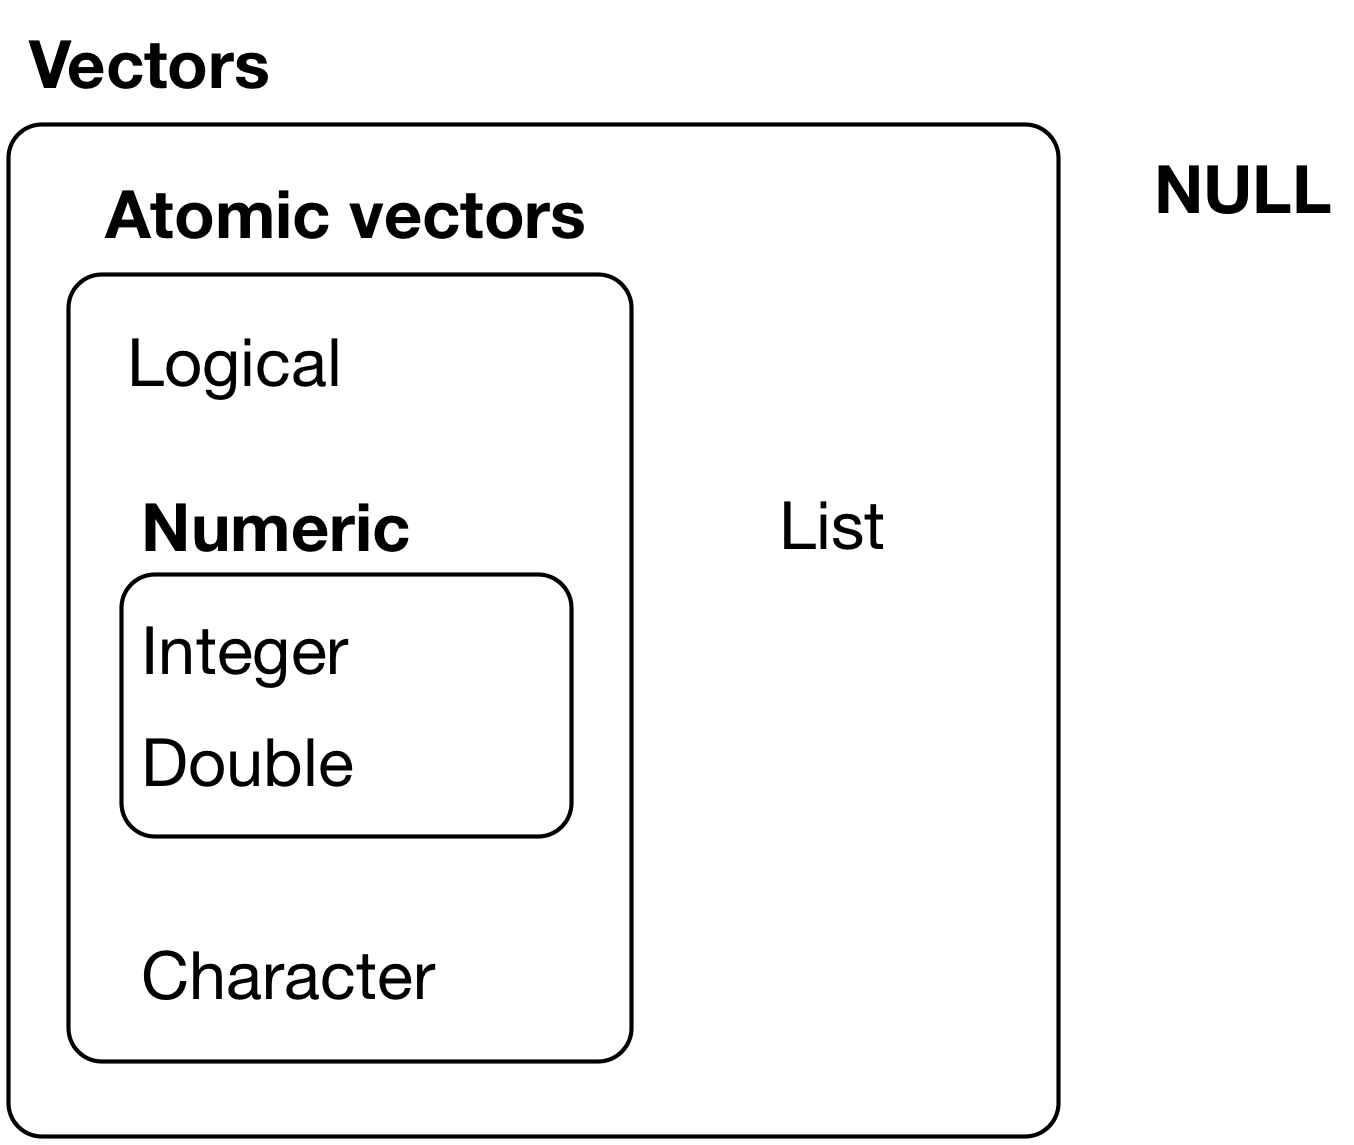
\includegraphics{./images/vector_hierarchy.png}
\caption{20.1}
\end{figure}

Every vector has two key properties:

\begin{enumerate}
\def\labelenumi{\arabic{enumi}.}
\item
  Its \textbf{type}, which you can determine with \texttt{typeof()}.

\begin{Shaded}
\begin{Highlighting}[]
\KeywordTok{typeof}\NormalTok{(letters)}
\end{Highlighting}
\end{Shaded}

\begin{verbatim}
## [1] "character"
\end{verbatim}

\begin{Shaded}
\begin{Highlighting}[]
\KeywordTok{typeof}\NormalTok{(}\DecValTok{1}\OperatorTok{:}\DecValTok{10}\NormalTok{)}
\end{Highlighting}
\end{Shaded}

\begin{verbatim}
## [1] "integer"
\end{verbatim}
\item
  Its \textbf{length}, which you can determine with \texttt{length()}.

\begin{Shaded}
\begin{Highlighting}[]
\NormalTok{x <-}\StringTok{ }\KeywordTok{list}\NormalTok{(}\StringTok{"a"}\NormalTok{, }\StringTok{"b"}\NormalTok{, }\DecValTok{1}\OperatorTok{:}\DecValTok{10}\NormalTok{)}
\KeywordTok{length}\NormalTok{(x)}
\end{Highlighting}
\end{Shaded}

\begin{verbatim}
## [1] 3
\end{verbatim}
\end{enumerate}

This chapter will introduce you to these important vectors from simplest to most complicated. You'll start with atomic vectors, then build up to lists, and finish off with augmented vectors.

\hypertarget{important-types-of-atomic-vector}{%
\section{Important types of atomic vector}\label{important-types-of-atomic-vector}}

The four most important types of atomic vector are logical, integer, double, and character.

\hypertarget{logical}{%
\section{Logical}\label{logical}}

Logical vectors are the simplest type of atomic vector because they can take only three possible values: \texttt{FALSE}, \texttt{TRUE}, and \texttt{NA}.\\
Logical vectors are usually constructed with comparison operators, you can also create them by hand with \texttt{c()}:

\begin{Shaded}
\begin{Highlighting}[]
\DecValTok{1}\OperatorTok{:}\DecValTok{10} \OperatorTok\StringTok{ }\DecValTok{3} \OperatorTok{==}\StringTok{ }\DecValTok{0}
\end{Highlighting}
\end{Shaded}

\begin{verbatim}
##  [1] FALSE FALSE  TRUE FALSE FALSE  TRUE FALSE FALSE  TRUE FALSE
\end{verbatim}

\begin{Shaded}
\begin{Highlighting}[]
\KeywordTok{c}\NormalTok{(}\OtherTok{TRUE}\NormalTok{, }\OtherTok{TRUE}\NormalTok{, }\OtherTok{FALSE}\NormalTok{, }\OtherTok{NA}\NormalTok{)}
\end{Highlighting}
\end{Shaded}

\begin{verbatim}
## [1]  TRUE  TRUE FALSE    NA
\end{verbatim}

\hypertarget{numeric}{%
\section{Numeric}\label{numeric}}

Integer and double vectors are known collectively as numeric vectors. In R, numbers are doubles by default.
To make an integer, place an \texttt{L} after the number:

\begin{Shaded}
\begin{Highlighting}[]
\KeywordTok{typeof}\NormalTok{(}\DecValTok{1}\NormalTok{)}
\end{Highlighting}
\end{Shaded}

\begin{verbatim}
## [1] "double"
\end{verbatim}

\begin{Shaded}
\begin{Highlighting}[]
\KeywordTok{typeof}\NormalTok{(1L)}
\end{Highlighting}
\end{Shaded}

\begin{verbatim}
## [1] "integer"
\end{verbatim}

\begin{Shaded}
\begin{Highlighting}[]
\FloatTok{1.5}\NormalTok{L}
\end{Highlighting}
\end{Shaded}

\begin{verbatim}
## [1] 1.5
\end{verbatim}

The distinction between integers and doubles is not usually important, but there are two important differences that you should be aware of:

\begin{enumerate}
\def\labelenumi{\arabic{enumi}.}
\item
  Doubles are approximations.

  For example, what is square of the square root of two?

\begin{Shaded}
\begin{Highlighting}[]
\NormalTok{x <-}\StringTok{ }\KeywordTok{sqrt}\NormalTok{(}\DecValTok{2}\NormalTok{) }\OperatorTok{^}\StringTok{ }\DecValTok{2}
\NormalTok{x}
\end{Highlighting}
\end{Shaded}

\begin{verbatim}
## [1] 2
\end{verbatim}

\begin{Shaded}
\begin{Highlighting}[]
\NormalTok{x }\OperatorTok{-}\StringTok{ }\DecValTok{2}
\end{Highlighting}
\end{Shaded}

\begin{verbatim}
## [1] 4.440892e-16
\end{verbatim}
\end{enumerate}

This behaviour is common when working with floating point numbers: most calculations include some approximation error.

Instead of comparing floating point numbers using \texttt{==}, you should use \texttt{dplyr::near()} which allows for some numerical tolerance.

\begin{enumerate}
\def\labelenumi{\arabic{enumi}.}
\setcounter{enumi}{1}
\item
  Integers have one special value: \texttt{NA}, while doubles have four: \texttt{NA}, \texttt{NaN}, \texttt{Inf} and \texttt{-Inf}.
  All three special values \texttt{NaN}, \texttt{Inf} and \texttt{-Inf} can arise during division:

\begin{Shaded}
\begin{Highlighting}[]
\KeywordTok{c}\NormalTok{(}\OperatorTok{-}\DecValTok{1}\NormalTok{, }\DecValTok{0}\NormalTok{, }\DecValTok{1}\NormalTok{) }\OperatorTok{/}\StringTok{ }\DecValTok{0}
\end{Highlighting}
\end{Shaded}

\begin{verbatim}
## [1] -Inf  NaN  Inf
\end{verbatim}

  Avoid using \texttt{==} to check for these other special values.
  Instead use the helper functions \texttt{is.finite()}, \texttt{is.infinite()}, and \texttt{is.nan()}:

  \begin{longtable}[]{@{}lllll@{}}
  \toprule
  & 0 & Inf & NA & NaN\tabularnewline
  \midrule
  \endhead
  \texttt{is.finite()} & x & & &\tabularnewline
  \texttt{is.infinite()} & & x & &\tabularnewline
  \texttt{is.na()} & & & x & x\tabularnewline
  \texttt{is.nan()} & & & & x\tabularnewline
  \bottomrule
  \end{longtable}
\end{enumerate}

\hypertarget{character}{%
\section{Character}\label{character}}

Character vectors are the most complex type of atomic vector, because each element of a character vector is a string, and a string can contain an arbitrary amount of data.

\texttt{parse\_number} function. (One of several parse functions.) Could be quite handy.

\begin{Shaded}
\begin{Highlighting}[]
\KeywordTok{parse_number}\NormalTok{(}\KeywordTok{c}\NormalTok{(}\StringTok{"1.0"}\NormalTok{, }\StringTok{"3.5"}\NormalTok{, }\StringTok{"$1,000.00"}\NormalTok{, }\StringTok{"NA"}\NormalTok{, }\StringTok{"ABCD12234.90"}\NormalTok{, }\StringTok{"1234ABC"}\NormalTok{, }\StringTok{"A123B"}\NormalTok{, }\StringTok{"A1B2C"}\NormalTok{))}
\end{Highlighting}
\end{Shaded}

\begin{verbatim}
## [1]     1.0     3.5  1000.0      NA 12234.9  1234.0   123.0     1.0
\end{verbatim}

You've already seen the most important type of implicit coercion: using a logical vector in a numeric context. In this case \texttt{TRUE} is converted to \texttt{1} and \texttt{FALSE} converted to \texttt{0}.
That means the sum of a logical vector is the number of \texttt{TRUE}s, and the mean of a logical vector is the proportion of \texttt{TRUE}s:

(Also one of the first times I've seen \texttt{sample()} in this document.)

\begin{Shaded}
\begin{Highlighting}[]
\NormalTok{x <-}\StringTok{ }\KeywordTok{sample}\NormalTok{(}\DecValTok{20}\NormalTok{, }\DecValTok{100}\NormalTok{, }\DataTypeTok{replace =} \OtherTok{TRUE}\NormalTok{) }\CommentTok{# sample integers from 1-20, 100 times w/replacement}
\NormalTok{y <-}\StringTok{ }\NormalTok{x }\OperatorTok{>}\StringTok{ }\DecValTok{10} \CommentTok{# create a logical vector (I think it's a vector)}
\KeywordTok{sum}\NormalTok{(y)  }\CommentTok{# how many are greater than 10?}
\end{Highlighting}
\end{Shaded}

\begin{verbatim}
## [1] 49
\end{verbatim}

\begin{Shaded}
\begin{Highlighting}[]
\KeywordTok{mean}\NormalTok{(y) }\CommentTok{# what proportion are greater than 10?}
\end{Highlighting}
\end{Shaded}

\begin{verbatim}
## [1] 0.49
\end{verbatim}

\hypertarget{scalars-and-recycling-rules}{%
\section{Scalars and recycling rules}\label{scalars-and-recycling-rules}}

As well as implicitly coercing the types of vectors to be compatible, R will also implicitly coerce the length of vectors.
This is called vector \textbf{recycling}, because the shorter vector is repeated, or recycled, to the same length as the longer vector.

This is generally most useful when you are mixing vectors and ``scalars''.

Because there are no scalars, most built-in functions are \textbf{vectorised}, meaning that they will operate on a vector of numbers.
That's why, for example, this code works:

\begin{Shaded}
\begin{Highlighting}[]
\KeywordTok{sample}\NormalTok{(}\DecValTok{10}\NormalTok{) }\OperatorTok{+}\StringTok{ }\DecValTok{100}
\end{Highlighting}
\end{Shaded}

\begin{verbatim}
##  [1] 110 101 103 108 106 102 109 105 107 104
\end{verbatim}

\begin{Shaded}
\begin{Highlighting}[]
\KeywordTok{runif}\NormalTok{(}\DecValTok{10}\NormalTok{) }\OperatorTok{>}\StringTok{ }\FloatTok{0.5}
\end{Highlighting}
\end{Shaded}

\begin{verbatim}
##  [1] FALSE FALSE FALSE  TRUE  TRUE FALSE  TRUE FALSE  TRUE  TRUE
\end{verbatim}

\begin{Shaded}
\begin{Highlighting}[]
\DecValTok{5}\OperatorTok{*}\KeywordTok{sample}\NormalTok{(}\DecValTok{5}\NormalTok{,}\DecValTok{10}\NormalTok{,}\DataTypeTok{replace=}\OtherTok{TRUE}\NormalTok{)}
\end{Highlighting}
\end{Shaded}

\begin{verbatim}
##  [1] 10 15 20 20  5 25  5 25 25  5
\end{verbatim}

\texttt{runif} is not a conditional \texttt{if} statement. It is a \texttt{r}andom draw from the {[}0,1{]} (\texttt{u}niform) interval.

\hypertarget{naming-vectors}{%
\section{Naming vectors}\label{naming-vectors}}

All types of vectors can be named.
You can name them during creation with \texttt{c()}:

\begin{Shaded}
\begin{Highlighting}[]
\KeywordTok{c}\NormalTok{(}\DataTypeTok{x =} \DecValTok{1}\NormalTok{, }\DataTypeTok{y =} \DecValTok{2}\NormalTok{, }\DataTypeTok{z =} \DecValTok{4}\NormalTok{)}
\end{Highlighting}
\end{Shaded}

\begin{verbatim}
## x y z 
## 1 2 4
\end{verbatim}

Or after the fact with \texttt{purrr::set\_names()}:

\begin{Shaded}
\begin{Highlighting}[]
\KeywordTok{set_names}\NormalTok{(}\DecValTok{1}\OperatorTok{:}\DecValTok{3}\NormalTok{, }\KeywordTok{c}\NormalTok{(}\StringTok{"a"}\NormalTok{, }\StringTok{"b"}\NormalTok{, }\StringTok{"c"}\NormalTok{))}
\end{Highlighting}
\end{Shaded}

\begin{verbatim}
## a b c 
## 1 2 3
\end{verbatim}

Named vectors are most useful for subsetting, described next.

\hypertarget{vector-subsetting}{%
\section{Subsetting}\label{vector-subsetting}}

So far we've used \texttt{dplyr::filter()} to filter the rows in a tibble.
\texttt{filter()} only works with tibble, so we'll need a new tool for vectors: \texttt{{[}}.
\texttt{{[}} is the subsetting function, and is called like \texttt{x{[}a{]}}.

There are four types of things that you can subset a vector with:

\begin{enumerate}
\def\labelenumi{\arabic{enumi}.}
\item
  A numeric vector containing only integers.
  The integers must either be all positive, all negative, or zero.

  Subsetting with positive integers keeps the elements at those positions:

\begin{Shaded}
\begin{Highlighting}[]
\NormalTok{x <-}\StringTok{ }\KeywordTok{c}\NormalTok{(}\StringTok{"one"}\NormalTok{, }\StringTok{"two"}\NormalTok{, }\StringTok{"three"}\NormalTok{, }\StringTok{"four"}\NormalTok{, }\StringTok{"five"}\NormalTok{)}
\NormalTok{x[}\KeywordTok{c}\NormalTok{(}\DecValTok{3}\NormalTok{, }\DecValTok{2}\NormalTok{, }\DecValTok{5}\NormalTok{)]}
\end{Highlighting}
\end{Shaded}

\begin{verbatim}
## [1] "three" "two"   "five"
\end{verbatim}

  By repeating a position, you can actually make a longer output than input:

\begin{Shaded}
\begin{Highlighting}[]
\NormalTok{x[}\KeywordTok{c}\NormalTok{(}\DecValTok{1}\NormalTok{, }\DecValTok{1}\NormalTok{, }\DecValTok{5}\NormalTok{, }\DecValTok{5}\NormalTok{, }\DecValTok{5}\NormalTok{, }\DecValTok{2}\NormalTok{)]}
\end{Highlighting}
\end{Shaded}

\begin{verbatim}
## [1] "one"  "one"  "five" "five" "five" "two"
\end{verbatim}

  Negative values drop the elements at the specified positions:

\begin{Shaded}
\begin{Highlighting}[]
\NormalTok{x[}\KeywordTok{c}\NormalTok{(}\OperatorTok{-}\DecValTok{1}\NormalTok{, }\DecValTok{-3}\NormalTok{, }\DecValTok{-5}\NormalTok{)]}
\end{Highlighting}
\end{Shaded}

\begin{verbatim}
## [1] "two"  "four"
\end{verbatim}

  It's an error to mix positive and negative values:

\begin{Shaded}
\begin{Highlighting}[]
\NormalTok{x[}\KeywordTok{c}\NormalTok{(}\DecValTok{1}\NormalTok{, }\DecValTok{-1}\NormalTok{)]}
\end{Highlighting}
\end{Shaded}

\begin{verbatim}
## Error in x[c(1, -1)]: only 0's may be mixed with negative subscripts
\end{verbatim}
\item
  Subsetting with a logical vector keeps all values corresponding to a \texttt{TRUE} value.
  This is most often useful in conjunction with the comparison functions.

\begin{Shaded}
\begin{Highlighting}[]
\NormalTok{x <-}\StringTok{ }\KeywordTok{c}\NormalTok{(}\DecValTok{10}\NormalTok{, }\DecValTok{3}\NormalTok{, }\OtherTok{NA}\NormalTok{, }\DecValTok{5}\NormalTok{, }\DecValTok{8}\NormalTok{, }\DecValTok{1}\NormalTok{, }\OtherTok{NA}\NormalTok{)}
\CommentTok{# All non-missing values of x}
\NormalTok{x[}\OperatorTok{!}\KeywordTok{is.na}\NormalTok{(x)]}
\end{Highlighting}
\end{Shaded}

\begin{verbatim}
## [1] 10  3  5  8  1
\end{verbatim}

\begin{Shaded}
\begin{Highlighting}[]
\CommentTok{# All even (or missing!) values of x}
\NormalTok{x[x }\OperatorTok\StringTok{ }\DecValTok{2} \OperatorTok{==}\StringTok{ }\DecValTok{0}\NormalTok{]}
\end{Highlighting}
\end{Shaded}

\begin{verbatim}
## [1] 10 NA  8 NA
\end{verbatim}

\begin{Shaded}
\begin{Highlighting}[]
\CommentTok{# All even AND not missing values of x}
\NormalTok{x[x }\OperatorTok\StringTok{ }\DecValTok{2} \OperatorTok{==}\StringTok{ }\DecValTok{0} \OperatorTok{&}\StringTok{ }\OperatorTok{!}\KeywordTok{is.na}\NormalTok{(x)]}
\end{Highlighting}
\end{Shaded}

\begin{verbatim}
## [1] 10  8
\end{verbatim}
\item
  If you have a named vector, you can subset it with a character vector:

\begin{Shaded}
\begin{Highlighting}[]
\NormalTok{x <-}\StringTok{ }\KeywordTok{c}\NormalTok{(}\DataTypeTok{abc =} \DecValTok{1}\NormalTok{, }\DataTypeTok{def =} \DecValTok{2}\NormalTok{, }\DataTypeTok{xyz =} \DecValTok{5}\NormalTok{)}
\NormalTok{x[}\KeywordTok{c}\NormalTok{(}\StringTok{"xyz"}\NormalTok{, }\StringTok{"def"}\NormalTok{)]}
\end{Highlighting}
\end{Shaded}

\begin{verbatim}
## xyz def 
##   5   2
\end{verbatim}
\item
  The simplest type of subsetting is nothing, \texttt{x{[}{]}}, which returns the complete \texttt{x}.
  This is not useful for subsetting vectors, but it is useful when subsetting matrices (and other high dimensional structures) because it lets you select all the rows or all the columns, by leaving that index blank.
  For example, if \texttt{x} is 2d, \texttt{x{[}1,\ {]}} selects the first row and all the columns, and \texttt{x{[},\ -1{]}} selects all rows and all columns except the first. \emph{(NOTE TO SELF: This last one is quite different from python, and a little unintuitive.)}
\end{enumerate}

To learn more about the applications of subsetting, reading the ``Subsetting'' chapter of \emph{Advanced R}: \url{http://adv-r.had.co.nz/Subsetting.html\#applications}.

There is an important variation of \texttt{{[}} called \texttt{{[}{[}}.
\texttt{{[}{[}} only ever extracts a single element, and always drops names.
It's a good idea to use it whenever you want to make it clear that you're extracting a single item, as in a for loop.
The distinction between \texttt{{[}} and \texttt{{[}{[}} is most important for lists, as we'll see shortly.

\hypertarget{exercises}{%
\section{Exercises}\label{exercises}}

The expression \texttt{sum(!is.finite(x))} calculates the number of elements in the vector that are equal to missing (NA), not-a-number (NaN), or infinity (Inf).

I hadn't realized that NA = `missing' and NaN = `not-a-number' until now.

\hypertarget{exercise-1}{%
\subsection{Exercise 1}\label{exercise-1}}

Two uses for this exercise. One, it's one of my first exposures to \texttt{function()} and
the first two answers contrast \texttt{{[}{]}} from \texttt{{[}{[}{]}{]}}, which seem important and easy to
confuse.

\emph{Create functions that take a vector as input and returns the last value. Should you use {[} or {[}{[}?}

\begin{Shaded}
\begin{Highlighting}[]
\NormalTok{last_value <-}\StringTok{ }\ControlFlowTok{function}\NormalTok{(x) \{}
  \CommentTok{# check for case with no length}
  \ControlFlowTok{if}\NormalTok{ (}\KeywordTok{length}\NormalTok{(x)) \{}
\NormalTok{    x[[}\KeywordTok{length}\NormalTok{(x)]]}
\NormalTok{  \} }\ControlFlowTok{else}\NormalTok{ \{}
\NormalTok{    x}
\NormalTok{  \}}
\NormalTok{\}}
\KeywordTok{last_value}\NormalTok{(}\KeywordTok{numeric}\NormalTok{())}
\end{Highlighting}
\end{Shaded}

\begin{verbatim}
## numeric(0)
\end{verbatim}

\begin{Shaded}
\begin{Highlighting}[]
\KeywordTok{last_value}\NormalTok{(}\DecValTok{1}\NormalTok{)}
\end{Highlighting}
\end{Shaded}

\begin{verbatim}
## [1] 1
\end{verbatim}

\begin{Shaded}
\begin{Highlighting}[]
\KeywordTok{last_value}\NormalTok{(}\DecValTok{1}\OperatorTok{:}\DecValTok{10}\NormalTok{)}
\end{Highlighting}
\end{Shaded}

\begin{verbatim}
## [1] 10
\end{verbatim}

\hypertarget{exercise-2}{%
\subsection{Exercise 2}\label{exercise-2}}

\emph{Return the elements at even numbered positions.}

\begin{Shaded}
\begin{Highlighting}[]
\NormalTok{even_indices <-}\StringTok{ }\ControlFlowTok{function}\NormalTok{(x) \{}
  \ControlFlowTok{if}\NormalTok{ (}\KeywordTok{length}\NormalTok{(x)) \{}
\NormalTok{    x[}\KeywordTok{seq_along}\NormalTok{(x) }\OperatorTok\StringTok{ }\DecValTok{2} \OperatorTok{==}\StringTok{ }\DecValTok{0}\NormalTok{]}
\NormalTok{  \} }\ControlFlowTok{else}\NormalTok{ \{}
\NormalTok{    x}
\NormalTok{  \}}
\NormalTok{\}}
\KeywordTok{even_indices}\NormalTok{(}\KeywordTok{numeric}\NormalTok{())}
\end{Highlighting}
\end{Shaded}

\begin{verbatim}
## numeric(0)
\end{verbatim}

\begin{Shaded}
\begin{Highlighting}[]
\KeywordTok{even_indices}\NormalTok{(}\DecValTok{1}\NormalTok{)}
\end{Highlighting}
\end{Shaded}

\begin{verbatim}
## numeric(0)
\end{verbatim}

\begin{Shaded}
\begin{Highlighting}[]
\KeywordTok{even_indices}\NormalTok{(}\DecValTok{1}\OperatorTok{:}\DecValTok{10}\NormalTok{)}
\end{Highlighting}
\end{Shaded}

\begin{verbatim}
## [1]  2  4  6  8 10
\end{verbatim}

\begin{Shaded}
\begin{Highlighting}[]
\KeywordTok{even_indices}\NormalTok{(letters)}
\end{Highlighting}
\end{Shaded}

\begin{verbatim}
##  [1] "b" "d" "f" "h" "j" "l" "n" "p" "r" "t" "v" "x" "z"
\end{verbatim}

Great \href{https://stackoverflow.com/questions/13732062/what-are-examples-of-when-seq-along-works-but-seq-produces-unintended-results}{example} on stackoverflow of\texttt{seq}vs.\texttt{seq\_along}. It appears there's every reason to
use\texttt{seq\_along}instead as its behavior makes more sense.

\hypertarget{exercise-3-seq}{%
\subsection{\texorpdfstring{Exercise 3: \texttt{seq()}}{Exercise 3: seq()}}\label{exercise-3-seq}}

\emph{Creating a sequence in a vector:}

\begin{Shaded}
\begin{Highlighting}[]
\NormalTok{x <-}\StringTok{ }\KeywordTok{seq}\NormalTok{(}\DataTypeTok{from =} \DecValTok{10}\NormalTok{, }\DataTypeTok{to =} \DecValTok{40}\NormalTok{, }\DataTypeTok{by =} \DecValTok{10}\NormalTok{)}
\NormalTok{y <-}\StringTok{ }\KeywordTok{seq}\NormalTok{(}\DataTypeTok{from =} \DecValTok{1}\NormalTok{, }\DataTypeTok{to =} \DecValTok{4}\NormalTok{, }\DataTypeTok{by =} \DecValTok{1}\NormalTok{)}\OperatorTok{^}\DecValTok{2}
\NormalTok{x}
\end{Highlighting}
\end{Shaded}

\begin{verbatim}
## [1] 10 20 30 40
\end{verbatim}

\begin{Shaded}
\begin{Highlighting}[]
\NormalTok{y}
\end{Highlighting}
\end{Shaded}

\begin{verbatim}
## [1]  1  4  9 16
\end{verbatim}

\hypertarget{exercise-4-rep}{%
\subsection{\texorpdfstring{Exercise 4: \texttt{rep()}}{Exercise 4: rep()}}\label{exercise-4-rep}}

\emph{Repeating data in a vector:}

\begin{Shaded}
\begin{Highlighting}[]
\NormalTok{one_to_ten_}\DecValTok{1}\NormalTok{ <-}\StringTok{ }\KeywordTok{c}\NormalTok{(}\DecValTok{1}\NormalTok{, }\DecValTok{2}\NormalTok{, }\DecValTok{3}\NormalTok{, }\DecValTok{4}\NormalTok{, }\DecValTok{5}\NormalTok{, }\DecValTok{6}\NormalTok{, }\DecValTok{7}\NormalTok{, }\DecValTok{8}\NormalTok{, }\DecValTok{9}\NormalTok{, }\DecValTok{10}\NormalTok{)}
\NormalTok{one_to_ten_}\DecValTok{2}\NormalTok{ <-}\StringTok{ }\DecValTok{1}\OperatorTok{:}\DecValTok{10}
\NormalTok{ten_to_one <-}\StringTok{ }\DecValTok{10}\OperatorTok{:}\DecValTok{1}

\NormalTok{one_to_ten_}\DecValTok{1}
\end{Highlighting}
\end{Shaded}

\begin{verbatim}
##  [1]  1  2  3  4  5  6  7  8  9 10
\end{verbatim}

\begin{Shaded}
\begin{Highlighting}[]
\NormalTok{one_to_ten_}\DecValTok{2}
\end{Highlighting}
\end{Shaded}

\begin{verbatim}
##  [1]  1  2  3  4  5  6  7  8  9 10
\end{verbatim}

\begin{Shaded}
\begin{Highlighting}[]
\NormalTok{ten_to_one}
\end{Highlighting}
\end{Shaded}

\begin{verbatim}
##  [1] 10  9  8  7  6  5  4  3  2  1
\end{verbatim}

\emph{Using \texttt{rep}licate}

Two arguments: \texttt{times} or \texttt{each}:

\begin{Shaded}
\begin{Highlighting}[]
\NormalTok{letter_vector <-}\StringTok{ }\KeywordTok{c}\NormalTok{(}\StringTok{'a'}\NormalTok{, }\StringTok{'b'}\NormalTok{, }\StringTok{'c'}\NormalTok{)}

\KeywordTok{rep}\NormalTok{(letter_vector, }\DataTypeTok{times =} \DecValTok{3}\NormalTok{)}
\end{Highlighting}
\end{Shaded}

\begin{verbatim}
## [1] "a" "b" "c" "a" "b" "c" "a" "b" "c"
\end{verbatim}

\begin{Shaded}
\begin{Highlighting}[]
\KeywordTok{rep}\NormalTok{(letter_vector, }\DataTypeTok{each =} \DecValTok{3}\NormalTok{)}
\end{Highlighting}
\end{Shaded}

\begin{verbatim}
## [1] "a" "a" "a" "b" "b" "b" "c" "c" "c"
\end{verbatim}

\begin{Shaded}
\begin{Highlighting}[]
\KeywordTok{rep}\NormalTok{(}\DecValTok{1}\OperatorTok{:}\DecValTok{4}\NormalTok{, }\DataTypeTok{times =} \DecValTok{1}\OperatorTok{:}\DecValTok{4}\NormalTok{)}
\end{Highlighting}
\end{Shaded}

\begin{verbatim}
##  [1] 1 2 2 3 3 3 4 4 4 4
\end{verbatim}

\hypertarget{exercise-5-sampling-vectors}{%
\subsection{Exercise 5: Sampling vectors}\label{exercise-5-sampling-vectors}}

\emph{Draws from a normal distribution:}

n = 8 draws from a normal distribution with mean 100 and sd = 20

\begin{Shaded}
\begin{Highlighting}[]
\KeywordTok{rnorm}\NormalTok{(}\DataTypeTok{n =} \DecValTok{8}\NormalTok{, }\DataTypeTok{mean =} \DecValTok{100}\NormalTok{, }\DataTypeTok{sd =} \DecValTok{20}\NormalTok{)}
\end{Highlighting}
\end{Shaded}

\begin{verbatim}
## [1]  91.66626 100.87064  94.58470 103.17574 168.69782 127.99914  68.42672
## [8]  94.25809
\end{verbatim}

\emph{Draws from the uniform distribution}

\begin{Shaded}
\begin{Highlighting}[]
\NormalTok{draws <-}\StringTok{ }\KeywordTok{runif}\NormalTok{(}\DataTypeTok{n =} \DecValTok{1000}\NormalTok{, }\DataTypeTok{min =} \DecValTok{-1}\NormalTok{, }\DataTypeTok{max =} \DecValTok{9}\NormalTok{)}
\KeywordTok{hist}\NormalTok{(draws, }\DataTypeTok{col =} \StringTok{'black'}\NormalTok{)}
\end{Highlighting}
\end{Shaded}

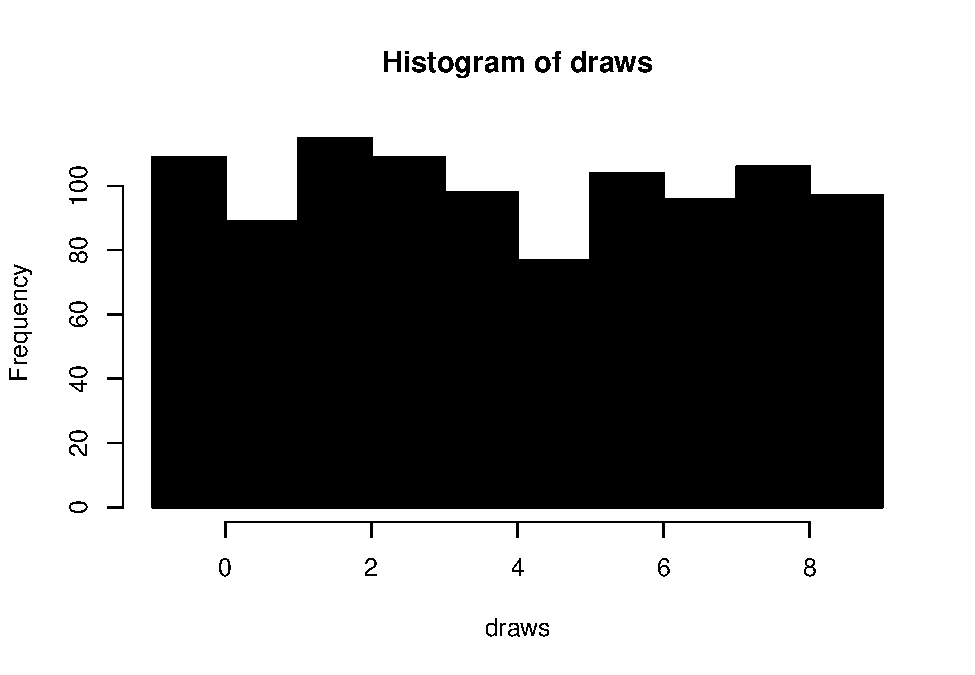
\includegraphics{Joes_R_Guide_files/figure-latex/unnamed-chunk-42-1.pdf}

\emph{Draw from a vector using the \texttt{sample()} function with or without replacement}

\begin{Shaded}
\begin{Highlighting}[]
\NormalTok{urn <-}\StringTok{ }\KeywordTok{c}\NormalTok{(}\StringTok{'red_ball'}\NormalTok{, }\StringTok{'blue_ball'}\NormalTok{, }\StringTok{'green_ball'}\NormalTok{)}
\KeywordTok{sample}\NormalTok{(}\DataTypeTok{x =}\NormalTok{ urn, }\DataTypeTok{size =} \DecValTok{4}\NormalTok{, }\DataTypeTok{replace =}\NormalTok{ T)}
\end{Highlighting}
\end{Shaded}

\begin{verbatim}
## [1] "red_ball"   "green_ball" "green_ball" "red_ball"
\end{verbatim}

\emph{To shuffle (makes use of default arguments):}

\begin{Shaded}
\begin{Highlighting}[]
\KeywordTok{sample}\NormalTok{(urn)}
\end{Highlighting}
\end{Shaded}

\begin{verbatim}
## [1] "green_ball" "blue_ball"  "red_ball"
\end{verbatim}

\hypertarget{exercise-6-make-a-matrix}{%
\subsection{\texorpdfstring{Exercise 6: Make a \texttt{matrix()}}{Exercise 6: Make a matrix()}}\label{exercise-6-make-a-matrix}}

\emph{Make a matrix:}

\begin{Shaded}
\begin{Highlighting}[]
\NormalTok{m <-}\StringTok{ }\KeywordTok{matrix}\NormalTok{(}\DataTypeTok{data =} \DecValTok{1}\OperatorTok{:}\DecValTok{10}\NormalTok{, }\DataTypeTok{ncol =} \DecValTok{2}\NormalTok{)}
\NormalTok{m}
\end{Highlighting}
\end{Shaded}

\begin{verbatim}
##      [,1] [,2]
## [1,]    1    6
## [2,]    2    7
## [3,]    3    8
## [4,]    4    9
## [5,]    5   10
\end{verbatim}

\begin{Shaded}
\begin{Highlighting}[]
\NormalTok{m[}\KeywordTok{c}\NormalTok{(}\DecValTok{1}\NormalTok{,}\DecValTok{2}\NormalTok{), }\KeywordTok{c}\NormalTok{(}\DecValTok{2}\NormalTok{,}\DecValTok{1}\NormalTok{)]}
\end{Highlighting}
\end{Shaded}

\begin{verbatim}
##      [,1] [,2]
## [1,]    6    1
## [2,]    7    2
\end{verbatim}

\hypertarget{lists}{%
\section{Recursive vectors (lists)}\label{lists}}

Lists are a step up in complexity from atomic vectors, because lists can contain other lists.
This makes them suitable for representing hierarchical or tree-like structures.
You create a list with \texttt{list()}:

\begin{Shaded}
\begin{Highlighting}[]
\NormalTok{x <-}\StringTok{ }\KeywordTok{list}\NormalTok{(}\DecValTok{1}\NormalTok{, }\DecValTok{2}\NormalTok{, }\DecValTok{3}\NormalTok{)}
\NormalTok{x}
\end{Highlighting}
\end{Shaded}

\begin{verbatim}
## [[1]]
## [1] 1
## 
## [[2]]
## [1] 2
## 
## [[3]]
## [1] 3
\end{verbatim}

A very useful tool for working with lists is \texttt{str()} because it focuses on the \textbf{str}ucture, not the contents.

\begin{Shaded}
\begin{Highlighting}[]
\NormalTok{y <-}\StringTok{ }\KeywordTok{list}\NormalTok{(}\StringTok{"a"}\NormalTok{, 1L, }\FloatTok{1.5}\NormalTok{, }\OtherTok{TRUE}\NormalTok{)}
\KeywordTok{str}\NormalTok{(y)}
\end{Highlighting}
\end{Shaded}

\begin{verbatim}
## List of 4
##  $ : chr "a"
##  $ : int 1
##  $ : num 1.5
##  $ : logi TRUE
\end{verbatim}

Lists can even contain other lists!

\begin{Shaded}
\begin{Highlighting}[]
\NormalTok{z <-}\StringTok{ }\KeywordTok{list}\NormalTok{(}\KeywordTok{list}\NormalTok{(}\DecValTok{1}\NormalTok{, }\DecValTok{2}\NormalTok{), }\KeywordTok{list}\NormalTok{(}\DecValTok{3}\NormalTok{, }\DecValTok{4}\NormalTok{))}
\KeywordTok{str}\NormalTok{(z)}
\end{Highlighting}
\end{Shaded}

\begin{verbatim}
## List of 2
##  $ :List of 2
##   ..$ : num 1
##   ..$ : num 2
##  $ :List of 2
##   ..$ : num 3
##   ..$ : num 4
\end{verbatim}

To explain more complicated list manipulation functions, it's helpful to have a visual representation of lists.
For example, take these three lists:

\begin{Shaded}
\begin{Highlighting}[]
\NormalTok{x1 <-}\StringTok{ }\KeywordTok{list}\NormalTok{(}\KeywordTok{c}\NormalTok{(}\DecValTok{1}\NormalTok{, }\DecValTok{2}\NormalTok{), }\KeywordTok{c}\NormalTok{(}\DecValTok{3}\NormalTok{, }\DecValTok{4}\NormalTok{))}
\NormalTok{x2 <-}\StringTok{ }\KeywordTok{list}\NormalTok{(}\KeywordTok{list}\NormalTok{(}\DecValTok{1}\NormalTok{, }\DecValTok{2}\NormalTok{), }\KeywordTok{list}\NormalTok{(}\DecValTok{3}\NormalTok{, }\DecValTok{4}\NormalTok{))}
\NormalTok{x3 <-}\StringTok{ }\KeywordTok{list}\NormalTok{(}\DecValTok{1}\NormalTok{, }\KeywordTok{list}\NormalTok{(}\DecValTok{2}\NormalTok{, }\KeywordTok{list}\NormalTok{(}\DecValTok{3}\NormalTok{)))}
\end{Highlighting}
\end{Shaded}

I'll draw them as follows:

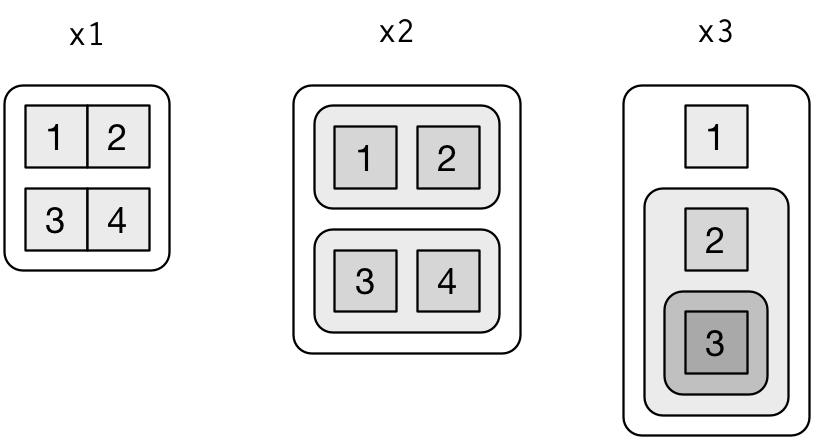
\includegraphics[width=0.5\linewidth]{./images/lists-structure}

\textbf{There are three principles:}

\begin{enumerate}
\def\labelenumi{\arabic{enumi}.}
\item
  Lists have rounded corners. Atomic vectors have square corners.
\item
  Children are drawn inside their parent, and have a slightly darker background to make it easier to see the hierarchy.
\item
  The orientation of the children (i.e.~rows or columns) isn't important, so I'll pick a row or column orientation to either save space or illustrate an important property in the example.
\end{enumerate}

\hypertarget{subsetting}{%
\subsection{Subsetting}\label{subsetting}}

There are three ways to subset a list, which I'll illustrate with a list named \texttt{a}:

\begin{Shaded}
\begin{Highlighting}[]
\NormalTok{a <-}\StringTok{ }\KeywordTok{list}\NormalTok{(}\DataTypeTok{a =} \DecValTok{1}\OperatorTok{:}\DecValTok{3}\NormalTok{, }\DataTypeTok{b =} \StringTok{"a string"}\NormalTok{, }\DataTypeTok{c =}\NormalTok{ pi, }\DataTypeTok{d =} \KeywordTok{list}\NormalTok{(}\OperatorTok{-}\DecValTok{1}\NormalTok{, }\DecValTok{-5}\NormalTok{))}
\end{Highlighting}
\end{Shaded}

\textbf{\texttt{{[}\ {]}} extracts a sub-list. The result will always be a list.}

\begin{Shaded}
\begin{Highlighting}[]
    \KeywordTok{str}\NormalTok{(a[}\DecValTok{1}\OperatorTok{:}\DecValTok{2}\NormalTok{])}
\end{Highlighting}
\end{Shaded}

\begin{verbatim}
## List of 2
##  $ a: int [1:3] 1 2 3
##  $ b: chr "a string"
\end{verbatim}

\begin{Shaded}
\begin{Highlighting}[]
    \KeywordTok{str}\NormalTok{(a[}\DecValTok{4}\NormalTok{])}
\end{Highlighting}
\end{Shaded}

\begin{verbatim}
## List of 1
##  $ d:List of 2
##   ..$ : num -1
##   ..$ : num -5
\end{verbatim}

As with vectors, you can subset with a logical, integer, or character vector. \textbf{\texttt{{[}{[}\ {]}{]}}extracts a single component from a list. It removes a level of hierarchy from the list.}

\begin{Shaded}
\begin{Highlighting}[]
    \KeywordTok{str}\NormalTok{(a[[}\DecValTok{1}\NormalTok{]])}
\end{Highlighting}
\end{Shaded}

\begin{verbatim}
##  int [1:3] 1 2 3
\end{verbatim}

\begin{Shaded}
\begin{Highlighting}[]
    \KeywordTok{str}\NormalTok{(a[[}\DecValTok{4}\NormalTok{]])}
\end{Highlighting}
\end{Shaded}

\begin{verbatim}
## List of 2
##  $ : num -1
##  $ : num -5
\end{verbatim}

\textbf{\texttt{\$}is a shorthand for extracting named elements of a list.} It works similarly to\texttt{{[}{[}\ {]}{]}}except that you don't need to use quotes.

\begin{Shaded}
\begin{Highlighting}[]
\NormalTok{  a}\OperatorTok{$}\NormalTok{a}
\end{Highlighting}
\end{Shaded}

\begin{verbatim}
## [1] 1 2 3
\end{verbatim}

\begin{Shaded}
\begin{Highlighting}[]
\NormalTok{  a[[}\StringTok{"a"}\NormalTok{]]}
\end{Highlighting}
\end{Shaded}

\begin{verbatim}
## [1] 1 2 3
\end{verbatim}

\hypertarget{more-vector-stuff}{%
\subsection{More vector stuff}\label{more-vector-stuff}}

\begin{Shaded}
\begin{Highlighting}[]
\NormalTok{v <-}\StringTok{ }\KeywordTok{c}\NormalTok{(}\DecValTok{1}\NormalTok{,}\DecValTok{2}\NormalTok{,}\DecValTok{3}\NormalTok{,}\DecValTok{4}\NormalTok{,}\DecValTok{6}\NormalTok{)}
\end{Highlighting}
\end{Shaded}

If a vector is one-dimensional, then we can either:

\begin{itemize}
\tightlist
\item
  Reference a location in that vector:

  \begin{itemize}
  \tightlist
  \item
    \texttt{v{[}2{]}} Will print the value in the second position
  \item
    \texttt{v{[}5{]}} Will print the value in the fifth position
  \item
    \texttt{v{[}c(2,5){]}} Will print the value in the second and fifth positions
  \item
    \texttt{v{[}-1{]}} Will print everything but the first \emph{note the difference between this and python}
  \end{itemize}
\item
  Pass a logical test that will print values

  \begin{itemize}
  \tightlist
  \item
    \texttt{v\ ==\ 2} Tests for each value in that vector taking a particular tested, in this case, 2.
  \end{itemize}
\end{itemize}

And so,

\begin{itemize}
\tightlist
\item
  \texttt{v{[}v\ ==\ 2{]}} Will print only the values that meet the test.
\item
  \texttt{v{[}v\ ==\ 6{]}} Will not print anything
\item
  \texttt{v{[}v\ \%in\%\ 1:3{]}} uses the set-based \texttt{\%in\%} operator which looks for existence in a range.
\end{itemize}

\begin{Shaded}
\begin{Highlighting}[]
\CommentTok{# returns by position}
\NormalTok{v[}\DecValTok{2}\NormalTok{]}
\end{Highlighting}
\end{Shaded}

\begin{verbatim}
## [1] 2
\end{verbatim}

\begin{Shaded}
\begin{Highlighting}[]
\NormalTok{v[}\DecValTok{5}\NormalTok{]}
\end{Highlighting}
\end{Shaded}

\begin{verbatim}
## [1] 6
\end{verbatim}

\begin{Shaded}
\begin{Highlighting}[]
\NormalTok{v[}\KeywordTok{c}\NormalTok{(}\DecValTok{2}\NormalTok{,}\DecValTok{5}\NormalTok{)]}
\end{Highlighting}
\end{Shaded}

\begin{verbatim}
## [1] 2 6
\end{verbatim}

\begin{Shaded}
\begin{Highlighting}[]
\CommentTok{# everything but the first position}
\NormalTok{v[}\OperatorTok{-}\DecValTok{1}\NormalTok{]}
\end{Highlighting}
\end{Shaded}

\begin{verbatim}
## [1] 2 3 4 6
\end{verbatim}

\begin{Shaded}
\begin{Highlighting}[]
\NormalTok{v }\OperatorTok{==}\StringTok{ }\DecValTok{2}
\end{Highlighting}
\end{Shaded}

\begin{verbatim}
## [1] FALSE  TRUE FALSE FALSE FALSE
\end{verbatim}

\begin{Shaded}
\begin{Highlighting}[]
\NormalTok{v[v }\OperatorTok{==}\StringTok{ }\DecValTok{2}\NormalTok{]}
\end{Highlighting}
\end{Shaded}

\begin{verbatim}
## [1] 2
\end{verbatim}

\begin{Shaded}
\begin{Highlighting}[]
\NormalTok{v }\OperatorTok\StringTok{ }\DecValTok{1}\OperatorTok{:}\DecValTok{3}
\end{Highlighting}
\end{Shaded}

\begin{verbatim}
## [1]  TRUE  TRUE  TRUE FALSE FALSE
\end{verbatim}

\begin{Shaded}
\begin{Highlighting}[]
\NormalTok{v[ v }\OperatorTok\StringTok{ }\DecValTok{1}\OperatorTok{:}\DecValTok{3}\NormalTok{ ]}
\end{Highlighting}
\end{Shaded}

\begin{verbatim}
## [1] 1 2 3
\end{verbatim}

The distinction between \texttt{{[}\ {]}} and \texttt{{[}{[}\ {]}{]}} is really important for lists, because \texttt{{[}{[}\ {]}{]}} drills down into the list while \texttt{{[}\ {]}} returns a new, smaller list.

\hypertarget{lists-of-condiments}{%
\subsection{Lists of condiments}\label{lists-of-condiments}}

The difference between \texttt{{[}} and \texttt{{[}{[}} is very important, but it's easy to get confused.
To help you remember, let me show you an unusual pepper shaker.


\includegraphics[width=0.25\linewidth]{images/pepper}

If this pepper shaker is your list \texttt{x}, then, \texttt{x{[}1{]}} is a pepper shaker containing a single pepper packet:

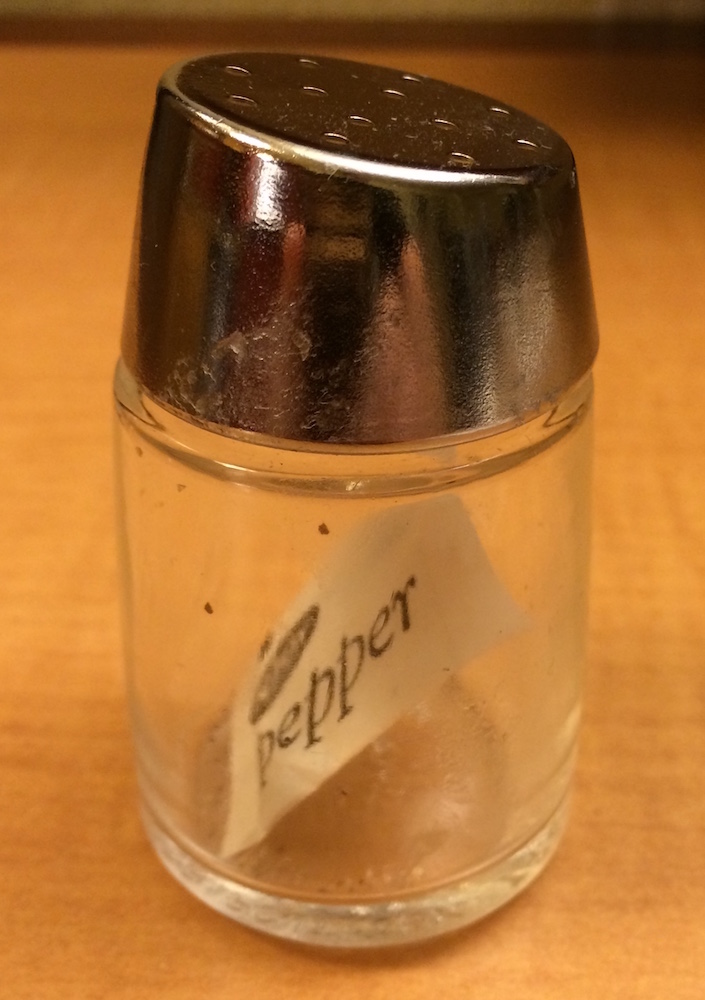
\includegraphics[width=0.25\linewidth]{images/pepper-1}

\texttt{x{[}2{]}} would look the same, but would contain the second packet.
\texttt{x{[}1:2{]}} would be a pepper shaker containing two pepper packets.

\texttt{x{[}{[}1{]}{]}} is:

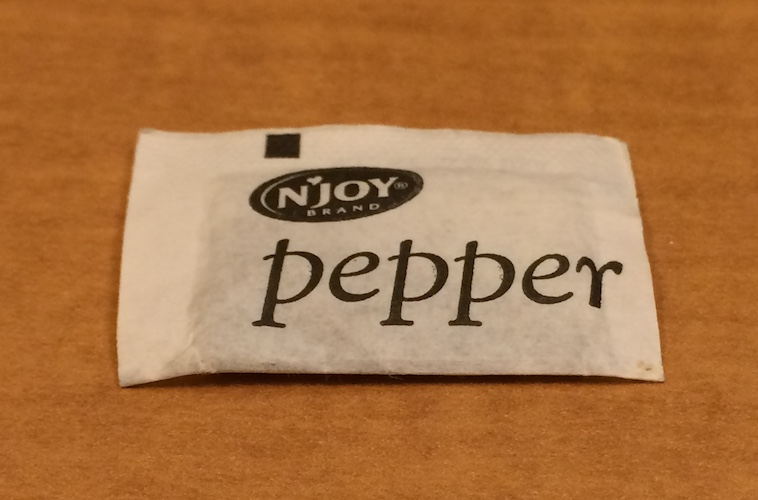
\includegraphics[width=0.25\linewidth]{images/pepper-2}

If you wanted to get the content of the pepper package, you'd need \texttt{x{[}{[}1{]}{]}{[}{[}1{]}{]}}:

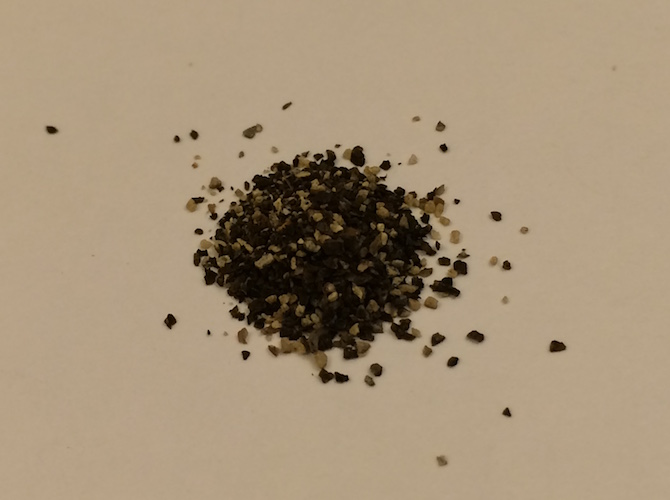
\includegraphics[width=0.25\linewidth]{images/pepper-3}

\hypertarget{augmented-vectors}{%
\section{Augmented vectors}\label{augmented-vectors}}

Atomic vectors and lists are the building blocks for other important vector types like factors and dates.
I call these \textbf{augmented vectors}, because they are vectors with additional \textbf{attributes}, including class.
Because augmented vectors have a class, they behave differently to the atomic vector on which they are built.
In this book, we make use of four important augmented vectors:

\begin{itemize}
\tightlist
\item
  Factors
\item
  Dates
\item
  Date-times
\item
  Tibbles
\end{itemize}

These are described below.

\hypertarget{dates-and-date-times}{%
\subsection{Dates and date-times}\label{dates-and-date-times}}

Dates in R are numeric vectors that represent the number of days since 1 January 1970.

\begin{Shaded}
\begin{Highlighting}[]
\NormalTok{x <-}\StringTok{ }\KeywordTok{as.Date}\NormalTok{(}\StringTok{"1971-01-01"}\NormalTok{)}
\KeywordTok{unclass}\NormalTok{(x)}
\end{Highlighting}
\end{Shaded}

\begin{verbatim}
## [1] 365
\end{verbatim}

\begin{Shaded}
\begin{Highlighting}[]
\KeywordTok{typeof}\NormalTok{(x)}
\end{Highlighting}
\end{Shaded}

\begin{verbatim}
## [1] "double"
\end{verbatim}

\begin{Shaded}
\begin{Highlighting}[]
\KeywordTok{attributes}\NormalTok{(x)}
\end{Highlighting}
\end{Shaded}

\begin{verbatim}
## $class
## [1] "Date"
\end{verbatim}

\hypertarget{methods}{%
\chapter{Methods}\label{methods}}

We describe our methods in this chapter.

\hypertarget{applications}{%
\chapter{Applications}\label{applications}}

Some \emph{significant} applications are demonstrated in this chapter.

\hypertarget{example-one}{%
\section{Example one}\label{example-one}}

\hypertarget{example-two}{%
\section{Example two}\label{example-two}}

\hypertarget{final-words}{%
\chapter{Final Words}\label{final-words}}

We have finished a nice book.

\hypertarget{dates}{%
\chapter{Dates}\label{dates}}

  \bibliography{book.bib,packages.bib}

\end{document}
